% 1977 年江苏盐城地区初试卷第七题：边长为 1 的正方形 ABCD 内作内接正方形 A1B1C1D1
% （按源卷第 2 页布局：A 左上、D 右上、C 右下、B 左下；A1 靠近 A、B1 靠近 B、C1 靠近 C、D1 靠近 D，图示取一般位置，非最小面积的特解）
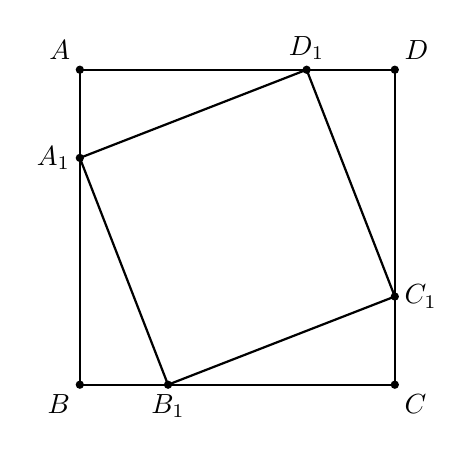
\begin{tikzpicture}[scale=1]
  \coordinate (A) at (0,4);
  \coordinate (B) at (0,0);
  \coordinate (C) at (4,0);
  \coordinate (D) at (4,4);
  \coordinate (A1) at (0,2.88);
  \coordinate (B1) at (1.12,0);
  \coordinate (C1) at (4,1.12);
  \coordinate (D1) at (2.88,4);
  \draw[thick] (A) -- (B) -- (C) -- (D) -- cycle;
  \draw[thick] (A1) -- (B1) -- (C1) -- (D1) -- cycle;
  \fill (A) circle (1.5pt) node[above left] {$A$};
  \fill (B) circle (1.5pt) node[below left] {$B$};
  \fill (C) circle (1.5pt) node[below right] {$C$};
  \fill (D) circle (1.5pt) node[above right] {$D$};
  \fill (A1) circle (1.5pt) node[left] {$A_1$};
  \fill (B1) circle (1.5pt) node[below] {$B_1$};
  \fill (C1) circle (1.5pt) node[right] {$C_1$};
  \fill (D1) circle (1.5pt) node[above] {$D_1$};
\end{tikzpicture}
